%!TEX TS-program = xelatex
%!TEX encoding = UTF-8 Unicode

\documentclass[a4paper]{article}

\usepackage{xltxtra}
\usepackage{amsfonts}
\usepackage{polyglossia}
\usepackage{fancyhdr}
\usepackage{geometry}
\usepackage{dsfont}
\usepackage{amsmath}
\usepackage{amsthm}
\usepackage{amssymb}
\usepackage{physics}
\usepackage{mathtools}
\usepackage{float}
\usepackage[shortlabels]{enumitem}

\geometry{a4paper,left=15mm,right=15mm,top=20mm,bottom=20mm}
\pagestyle{fancy}
\lhead{Devon Morris}
\chead{Dynamics}
\rhead{\today}
\cfoot{\thepage}

\setlength{\headheight}{23pt}
\setlength{\parindent}{0.0in}
\setlength{\parskip}{0.0in}

\newtheorem*{prop}{Proposition}
\newtheorem*{defn}{Definition}
\newtheorem*{thm}{Theorem}
\newtheorem*{cor}{Corollary}
\newtheorem*{lem}{Lemma}
\newtheorem*{rem}{Remark}

\DeclarePairedDelimiterX{\inn}[2]{\langle}{\rangle}{#1, #2}

\begin{document}
\section*{Final Project: Apollo Spacecraft Attitude Dynamics}%

\subsection*{Task A:}%
Let $\hat{i}$, $\hat{j}$, $\hat{k}$ be the unit vectors of the $A$ frame.
\begin{enumerate}[a.]
  \item General Case:
    The location of the center of mass is
    \[
      r_{G/A} = 23.6177 \hat{i} + 0.0961 \hat{j} + -0.0087 \hat{k}\ m
    \]
    which gives us the inertia matrix of
    \[
      \begin{aligned}
        [I_{G/A}] &= [I_{SM/A}] + [I_{CM/A}] + [I_{PROP/A}] \\
                  &= 
                  \begin{bmatrix}
                    I_{xx} & -I_{xy} & -I_{xz} \\
                    -I_{xy} & I_{yy} & -I_{yz} \\
                    -I_{xz} & -I_{yz} & I_{zz}
                  \end{bmatrix} \\
            &=
            \begin{bmatrix}
              40823.073 &  1537.807 & -3179.297 \\
              1537.807 & 90593.489 & 128.577 \\
              -3179.297 & 128.577 & 98742.852
            \end{bmatrix}
      \end{aligned}
    \]
  \item Simplified Case:
    The location of the center of mass is
    \[
      r_{G/A} = 23.6177 \hat{i}\ m
    \]
    which gives us the inertia matrix of
    \[
      [I_{G/A}] = 
      \begin{bmatrix}
        40481.983 & 0 & 0 \\
        0 & 90358.316 & 0 \\
        0 & 0 & 98636.935
      \end{bmatrix}
    \]
\end{enumerate}

\subsection*{Task B:}%
First we have that the euler angle rates and angular velocities are related by
\[
  \begin{aligned}
    \omega_x &= - \dot{\psi} s_{\theta} + \dot{\phi} \\
    \omega_y &= \dot{\psi} c_{\theta}s_{\phi} + \dot{\theta} c_{\phi} \\
    \omega_z &= \dot{\psi}c_{\theta}c_{\phi} - \dot{\theta}s_{\phi}
  \end{aligned}
\]
and inversely
\[
  \begin{aligned}
    \dot{\psi} &= \frac{1}{c_{\theta}} \left( \omega_y s_{\phi} + \omega_z c_{\phi} \right) \\
    \dot{\theta} &= \omega_y c_{\phi} - \omega_z s_{\phi} \\
    \dot{\phi} &= \frac{1}{c_{\theta}} \left( \omega_y s_{\theta} s_{\phi} + \omega_z s_{\theta}c_{\phi} \right) + \omega_x
  \end{aligned}
\]
These can be coupled with the standard rotational equations of motion
\[
  \begin{aligned}
  I_{xx} \dot{\omega}_x - I_{xy} \left( \dot{\omega}_y - \omega_x \omega_z\right) - I_{xz}(\dot{\omega}_z + \omega_x \omega_y) - (I_{yy} - I_{zz})\omega_y \omega_z - I_{yz} (\omega_y^2 - \omega_z^2) = M_x \\
  I_{yy} \dot{\omega}_y - I_{yz} \left( \dot{\omega}_x - \omega_y \omega_z\right) - I_{xy}(\dot{\omega}_x + \omega_y \omega_z) - (I_{zz} - I_{xx})\omega_x \omega_z - I_{xz} (\omega_z^2 - \omega_x^2) = M_y \\
  I_{zz} \dot{\omega}_z - I_{xz} \left( \dot{\omega}_x - \omega_y \omega_z\right) - I_{yz}(\dot{\omega}_y + \omega_x \omega_z) - (I_{xx} - I_{yy})\omega_x \omega_y - I_{xy} (\omega_x^2 - \omega_y^2) = M_z \\
  \end{aligned}
\]
Additionally, we can write these rotational equations in terms of euler angles and their derivatives as
\[
  \begin{aligned}
    \dv{t} \left( \phi \right) =& \dot{\phi} \\ 
    \dv{t} \left( \theta \right) =& \dot{\theta} \\
    \dv{t} \left( \psi \right) =& \dot{\psi} \\
    M_x =& 
\left(-I_{xx}\,s_\theta-I_{xz}\,c_\phi\,c_\theta-I_{xy}\,c_\theta\,s_\phi\right)\,\ddot{\psi}+I_{xx}\,\ddot{\phi}+\left(I_{xz}\,s_\phi-I_{xy}\,c_\phi\right)\,\ddot{\theta} \\ 
         &+\left(I_{yz}\,{c_\phi}^2\,{c_\theta}^2-I_{yz}\,{c_\theta}^2\,{s_\phi}^2-I_{xy}\,c_\phi\,c_\theta\,s_\theta+I_{xz}\,c_\theta\,s_\phi\,s_\theta-I_{yy}\,c_\phi\,{c_\theta}^2\,s_\phi+I_{zz}\,c_\phi\,{c_\theta}^2\,s_\phi\right)\,{\dot{\psi}}^2 \\
         &+\left(2\,I_{xz}\,c_\phi\,s_\theta-I_{xx}\,c_\theta+2\,I_{xy}\,s_\phi\,s_\theta-I_{yy}\,{c_\phi}^2\,c_\theta+I_{zz}\,{c_\phi}^2\,c_\theta+I_{yy}\,c_\theta\,{s_\phi}^2-I_{zz}\,c_\theta\,{s_\phi}^2-4\,I_{yz}\,c_\phi\,c_\theta\,s_\phi\right)\,\dot{\psi}\,\dot{\theta} \\
         &+\left(I_{yz}\,{s_\phi}^2-I_{yz}\,{c_\phi}^2+I_{yy}\,c_\phi\,s_\phi-I_{zz}\,c_\phi\,s_\phi\right)\,{\dot{\theta}}^2 \\
    M_y =&
\left(I_{xy}\,s_\theta-I_{yz}\,c_\phi\,c_\theta+I_{yy}\,c_\theta\,s_\phi\right)\,\ddot{\psi}+\left(-I_{xy}\right)\,\ddot{\phi}+\left(I_{yy}\,c_\phi+I_{yz}\,s_\phi\right)\,\ddot{\theta} \\
         &+\left(I_{xz}\,{s_\theta}^2-I_{xz}\,{c_\phi}^2\,{c_\theta}^2-I_{xx}\,c_\phi\,c_\theta\,s_\theta+I_{zz}\,c_\phi\,c_\theta\,s_\theta-I_{yz}\,c_\theta\,s_\phi\,s_\theta-I_{xy}\,c_\phi\,{c_\theta}^2\,s_\phi\right)\,{\dot{\psi}}^2 \\
         &+\left(I_{xx}\,c_\phi\,c_\theta-2\,I_{xz}\,s_\theta+I_{yy}\,c_\phi\,c_\theta-I_{zz}\,c_\phi\,c_\theta+2\,I_{yz}\,c_\theta\,s_\phi\right)\,\dot{\psi}\,\dot{\phi} \\
         &+\left(I_{xy}\,c_\theta+I_{xx}\,s_\phi\,s_\theta-I_{yy}\,s_\phi\,s_\theta-I_{zz}\,s_\phi\,s_\theta-I_{xy}\,{c_\phi}^2\,c_\theta+I_{xy}\,c_\theta\,{s_\phi}^2+2\,I_{xz}\,c_\phi\,c_\theta\,s_\phi\right)\,\dot{\psi}\,\dot{\theta} \\
         &+I_{xz}\,{\dot{\phi}}^2+\left(2\,I_{yz}\,c_\phi-I_{xx}\,s_\phi-I_{yy}\,s_\phi+I_{zz}\,s_\phi\right)\,\dot{\phi}\,\dot{\theta}+\left(I_{xy}\,c_\phi\,s_\phi-I_{xz}\,{s_\phi}^2\right)\,{\dot{\theta}}^2 \\
    M_z =&
\left(I_{xz}\,s_\theta+I_{zz}\,c_\phi\,c_\theta-I_{yz}\,c_\theta\,s_\phi\right)\,\ddot{\psi}+\left(-I_{xz}\right)\,\ddot{\phi}+\left(-I_{yz}\,c_\phi-I_{zz}\,s_\phi\right)\,\ddot{\theta} \\
         &+\left(I_{xy}\,{c_\theta}^2\,{s_\phi}^2-I_{xy}\,{s_\theta}^2+I_{yz}\,c_\phi\,c_\theta\,s_\theta+I_{xx}\,c_\theta\,s_\phi\,s_\theta-I_{yy}\,c_\theta\,s_\phi\,s_\theta+I_{xz}\,c_\phi\,{c_\theta}^2\,s_\phi\right)\,{\dot{\psi}}^2 \\
         &+\left(2\,I_{xy}\,s_\theta-2\,I_{yz}\,c_\phi\,c_\theta-I_{xx}\,c_\theta\,s_\phi+I_{yy}\,c_\theta\,s_\phi-I_{zz}\,c_\theta\,s_\phi\right)\,\dot{\psi}\,\dot{\phi} \\
         &+\left(I_{xz}\,c_\theta+I_{xx}\,c_\phi\,s_\theta-I_{yy}\,c_\phi\,s_\theta-I_{zz}\,c_\phi\,s_\theta+I_{xz}\,{c_\phi}^2\,c_\theta-I_{xz}\,c_\theta\,{s_\phi}^2+2\,I_{xy}\,c_\phi\,c_\theta\,s_\phi\right)\,\dot{\psi}\,\dot{\theta} \\
         &-I_{xy}\,{\dot{\phi}}^2+\left(I_{yy}\,c_\phi-I_{xx}\,c_\phi-I_{zz}\,c_\phi+2\,I_{yz}\,s_\phi\right)\,\dot{\phi}\,\dot{\theta}+\left(I_{xy}\,{c_\phi}^2-I_{xz}\,c_\phi\,s_\phi\right)\,{\dot{\theta}}^2
  \end{aligned}
\]
\subsection*{Task C:}%
\begin{enumerate}[a.]
  \item  See attached \texttt{morris.m}
  \item  Here are the plots of the general case
    \begin{figure}[H]
    \begin{center}
      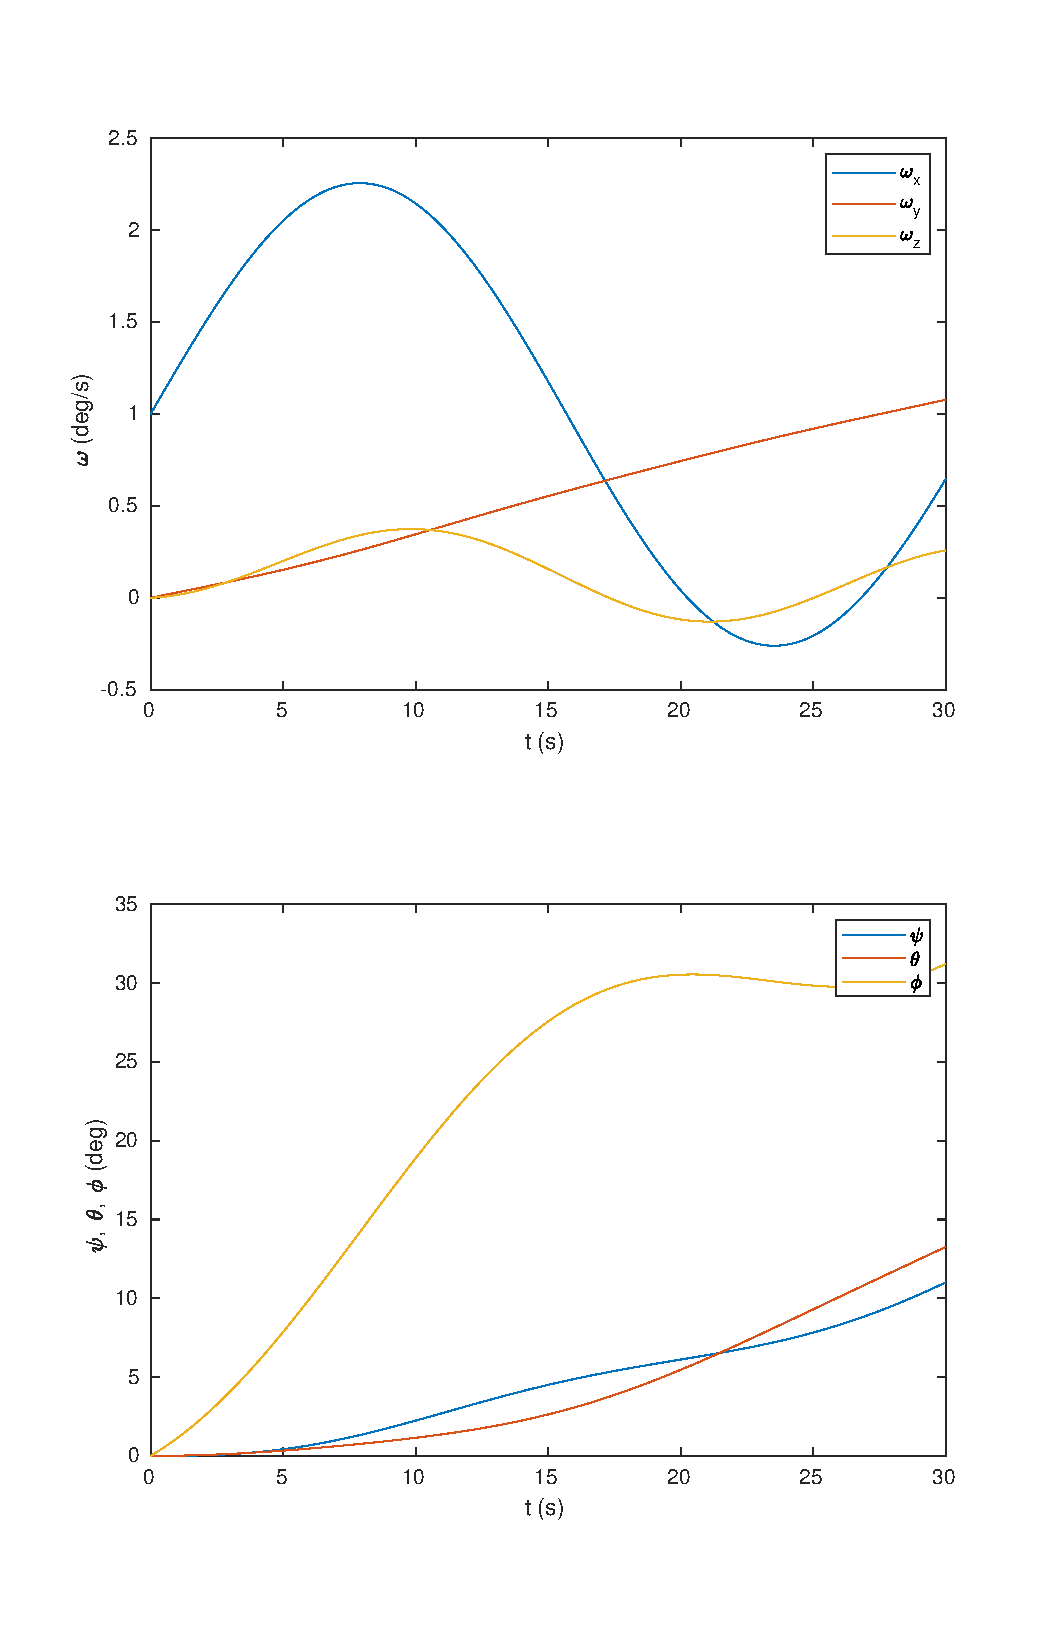
\includegraphics[scale=0.7]{task_c.eps}
    \end{center}
    \caption{Simulation of CSM attitude (General)}
    \label{fig:task_c}
    \end{figure}

    Here is a table of maximum and minimum values in the general case
    \begin{table}[H]
      \centering
      \begin{tabular}{lcccccc}
        & $\omega_x$ & $\omega_y$ & $\omega_z$ & $\psi$ & $\theta$ & $\phi$ \\
        $\max$ &  2.2554 & 1.0744 & 0.3740 & 11.0113 & 13.2593 & 31.2242\\
        $\min$ & -0.2605 & 0.0000 & -0.1293 & 0.0000 & 0.0000 & 0.0000 \\
      \end{tabular}
      \caption{Table of max and min values shown in degrees and degrees per second (General)}
    \end{table}

    \begin{figure}[H]
    \begin{center}
      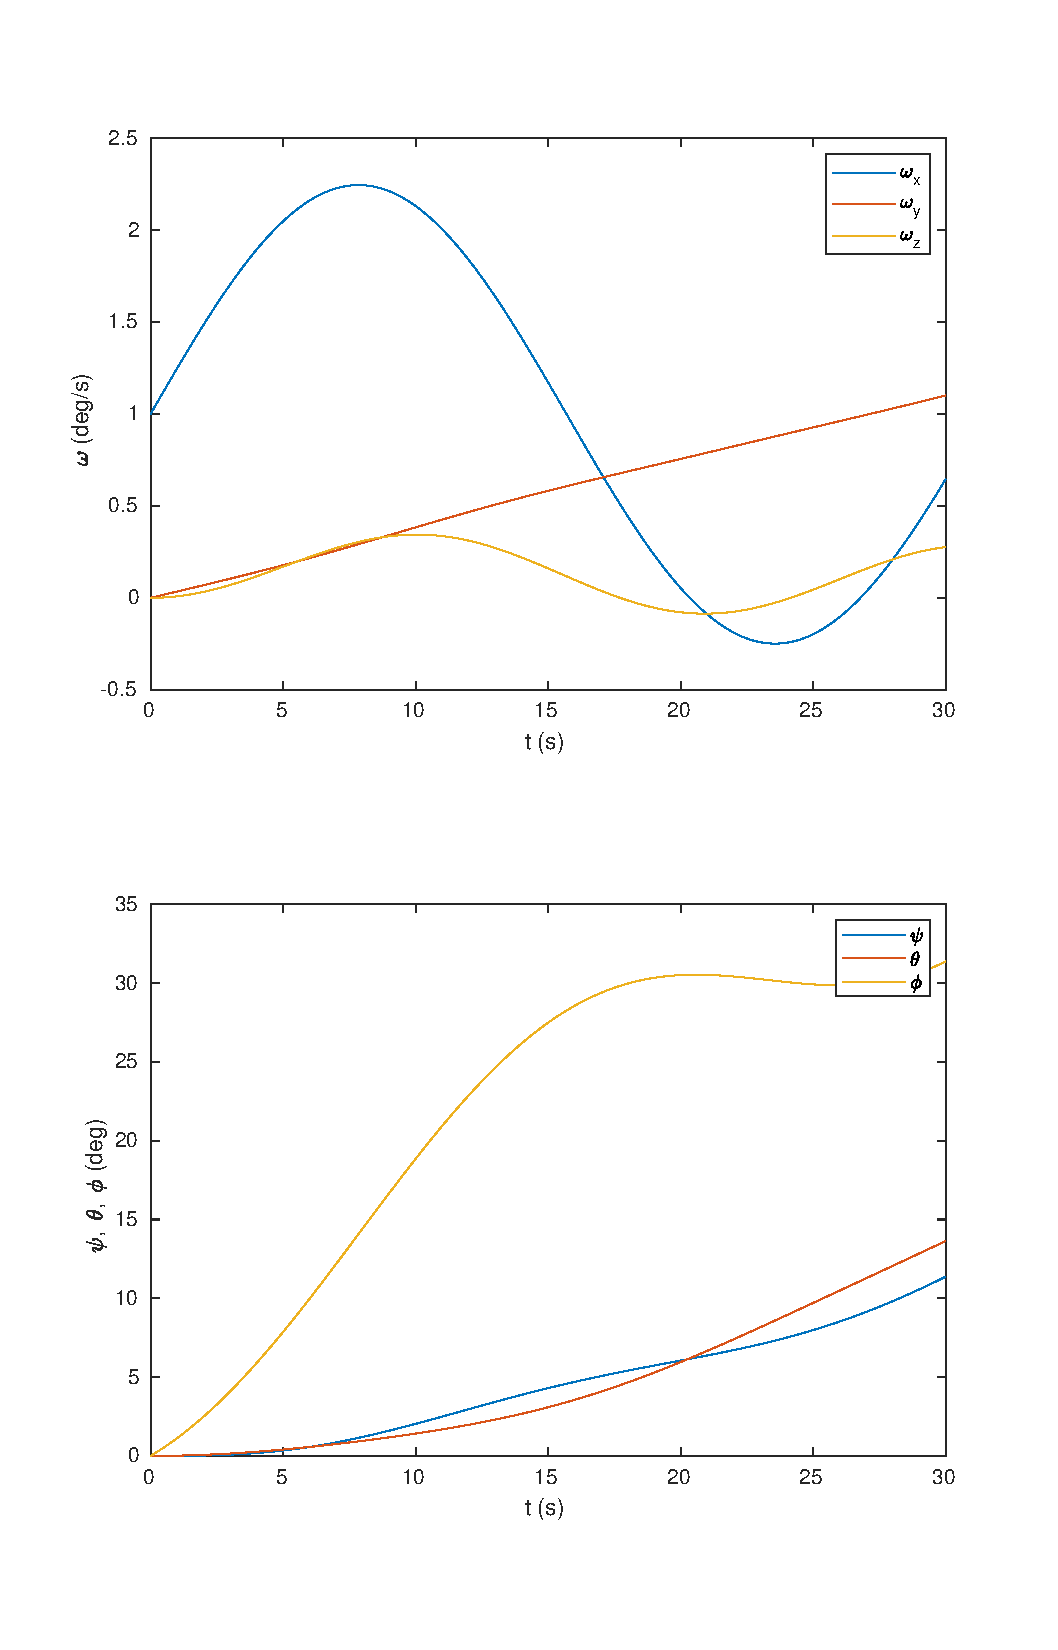
\includegraphics[scale=0.7]{task_c_simplified.eps}
    \end{center}
    \caption{Simulation of CSM attitude (Simplified)}
    \label{fig:task_c_simplified}
    \end{figure}

    Here is a table of maximum and minimum values in the simplified case
    \begin{table}[H]
      \centering
      \begin{tabular}{lcccccc}
        & $\omega_x$ & $\omega_y$ & $\omega_z$ & $\psi$ & $\theta$ & $\phi$ \\
        $\max$ &  2.2448 & 1.1006 & 0.3439 & 11.3695 & 13.6357 & 31.3756 \\
        $\min$ & -0.2489 & 0.0000 & -0.0859 & 0.0000 & 0.0000 & 0.0000 \\
      \end{tabular}
      \caption{Table of max and min values shown in degrees and degrees per second (Simplified)}
    \end{table}
  \item I calculated that the torques need to be
    \[
      \begin{aligned}
        M_x &= 0.000000\ Nm \\
        M_y &= 0.968469\ Nm\\
        M_z &= 0.468443\ Nm
      \end{aligned}
    \]
    When these torques are applied the following response is observed.
    \begin{figure}[H]
    \begin{center}
      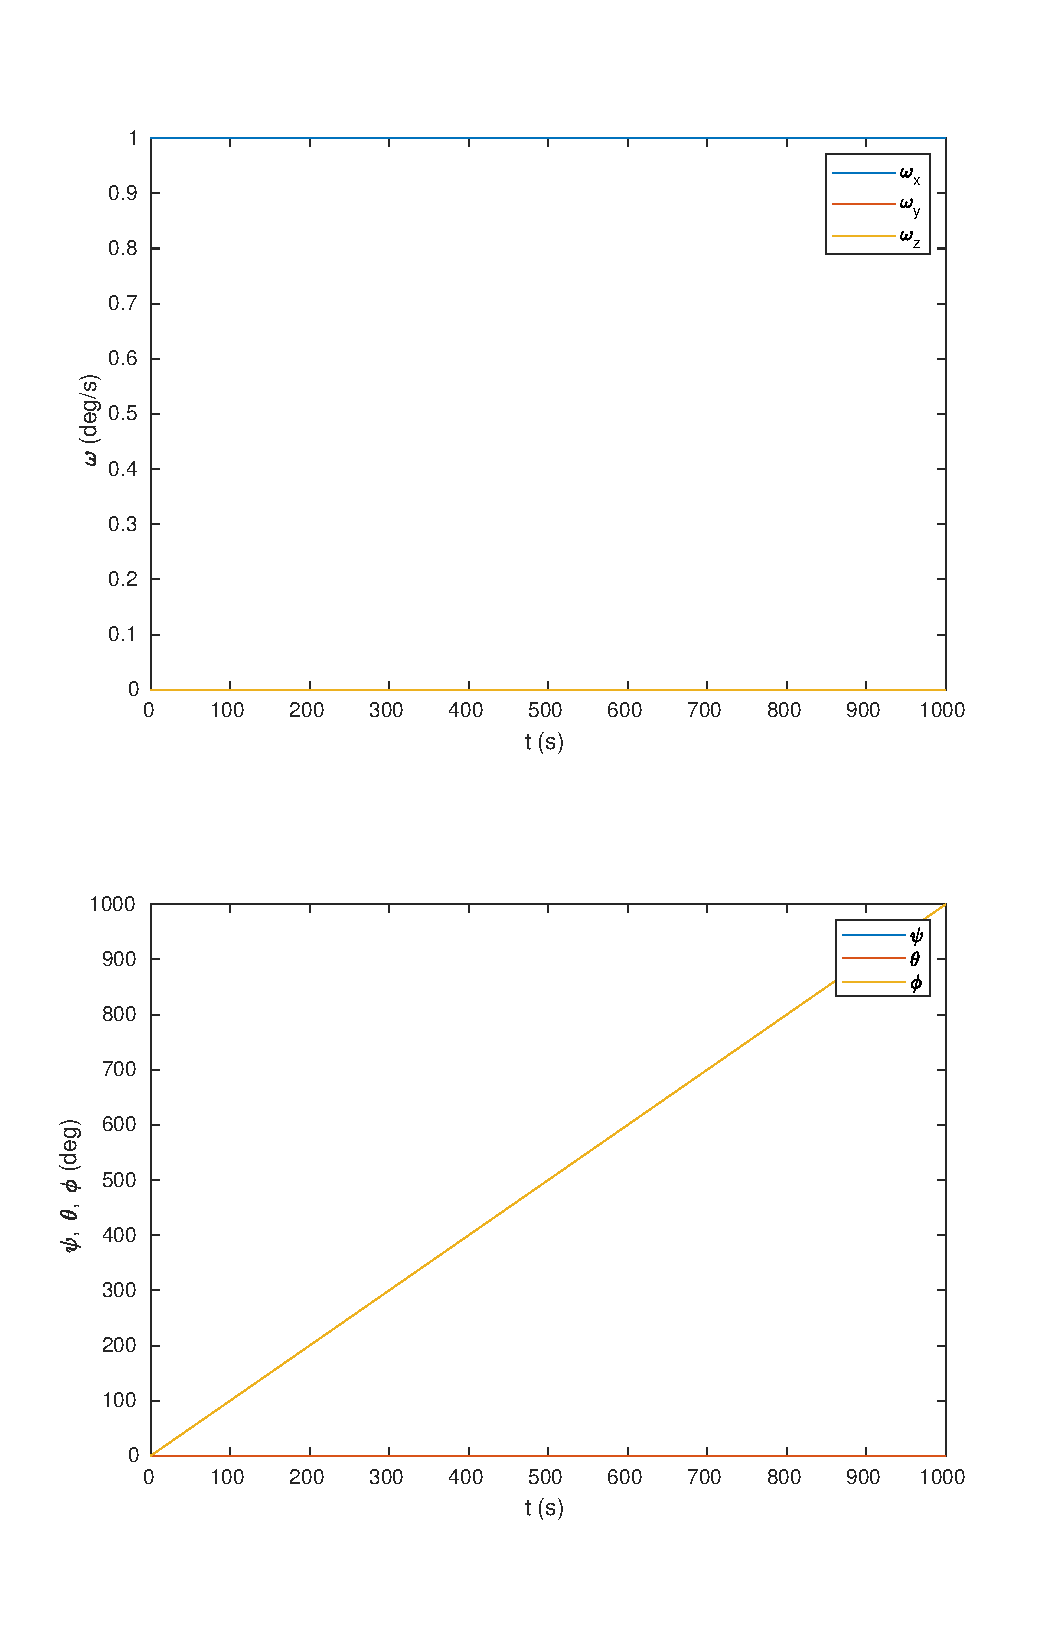
\includegraphics[scale=0.7]{task_c_torques.eps}
    \end{center}
    \caption{Simulation of CSM attitude with constant torques}
    \label{fig:task_c_torques}
    \end{figure}

    When no torques are applied the following response is observed
    \begin{figure}[H]
    \begin{center}
      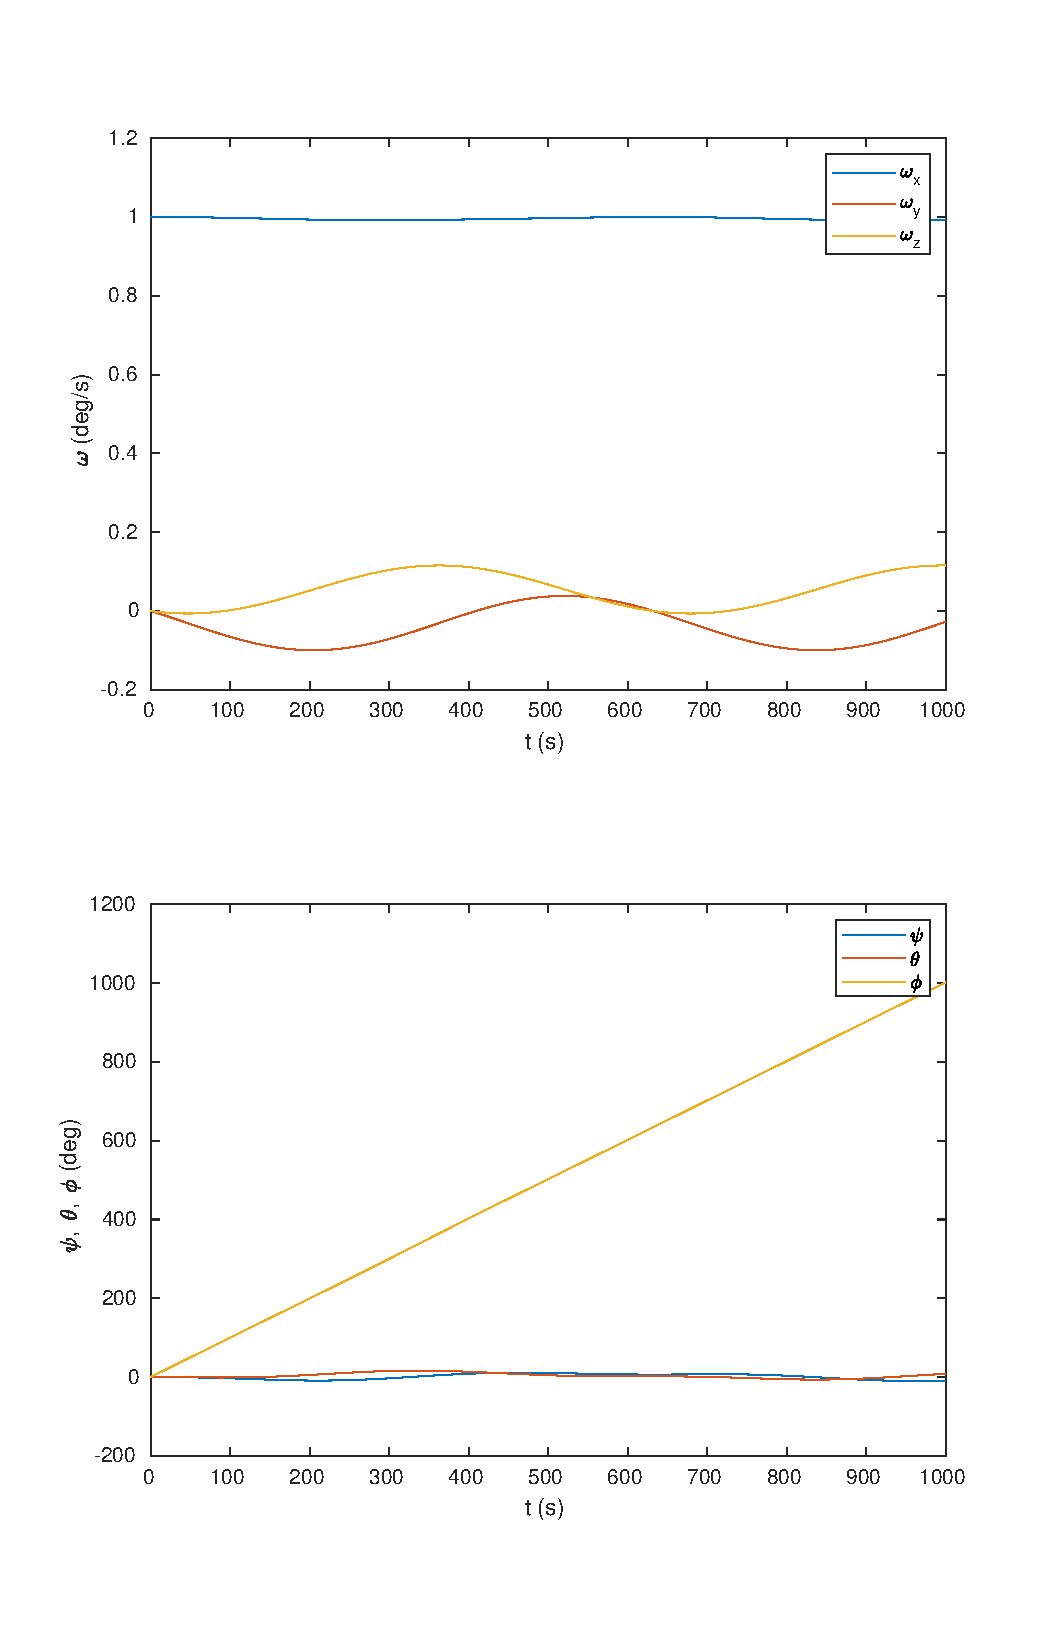
\includegraphics[scale=0.7]{task_c_no_torques.eps}
    \end{center}
    \caption{Simulation of CSM attitude with no applied torques}
    \label{fig:task_c_no_torques}
    \end{figure}
\end{enumerate}

\subsection*{Task D:}%
\begin{enumerate}[a.]
  \item  The moments induced by the CMGs on the aircraft are
    \[
      \begin{aligned}
        M_x &= -I_R \Omega(-s_{\theta_1} \dot{\theta}_1 + c_{\theta_3} \dot{\theta}_3)\\
        M_y &= -I_R \Omega(c_{\theta_1} \dot{\theta}_1 - s_{\theta_2} \dot{\theta}_2) \\
        M_z &= -I_R \Omega(c_{\theta_2} \dot{\theta}_2 - s_{\theta_3} \dot{\theta}_3)
      \end{aligned}
    \]
  \item In order to ensure the desired angular accelerations, 
    \[
      I_R \geq 11.9056
    \]
\end{enumerate}

\subsection*{Task E:}%
\begin{enumerate}[a.]
  \item See attached \texttt{morris\_cmg.m}
  \item The simulation results in the following motion
    \begin{figure}[H]
    \begin{center}
      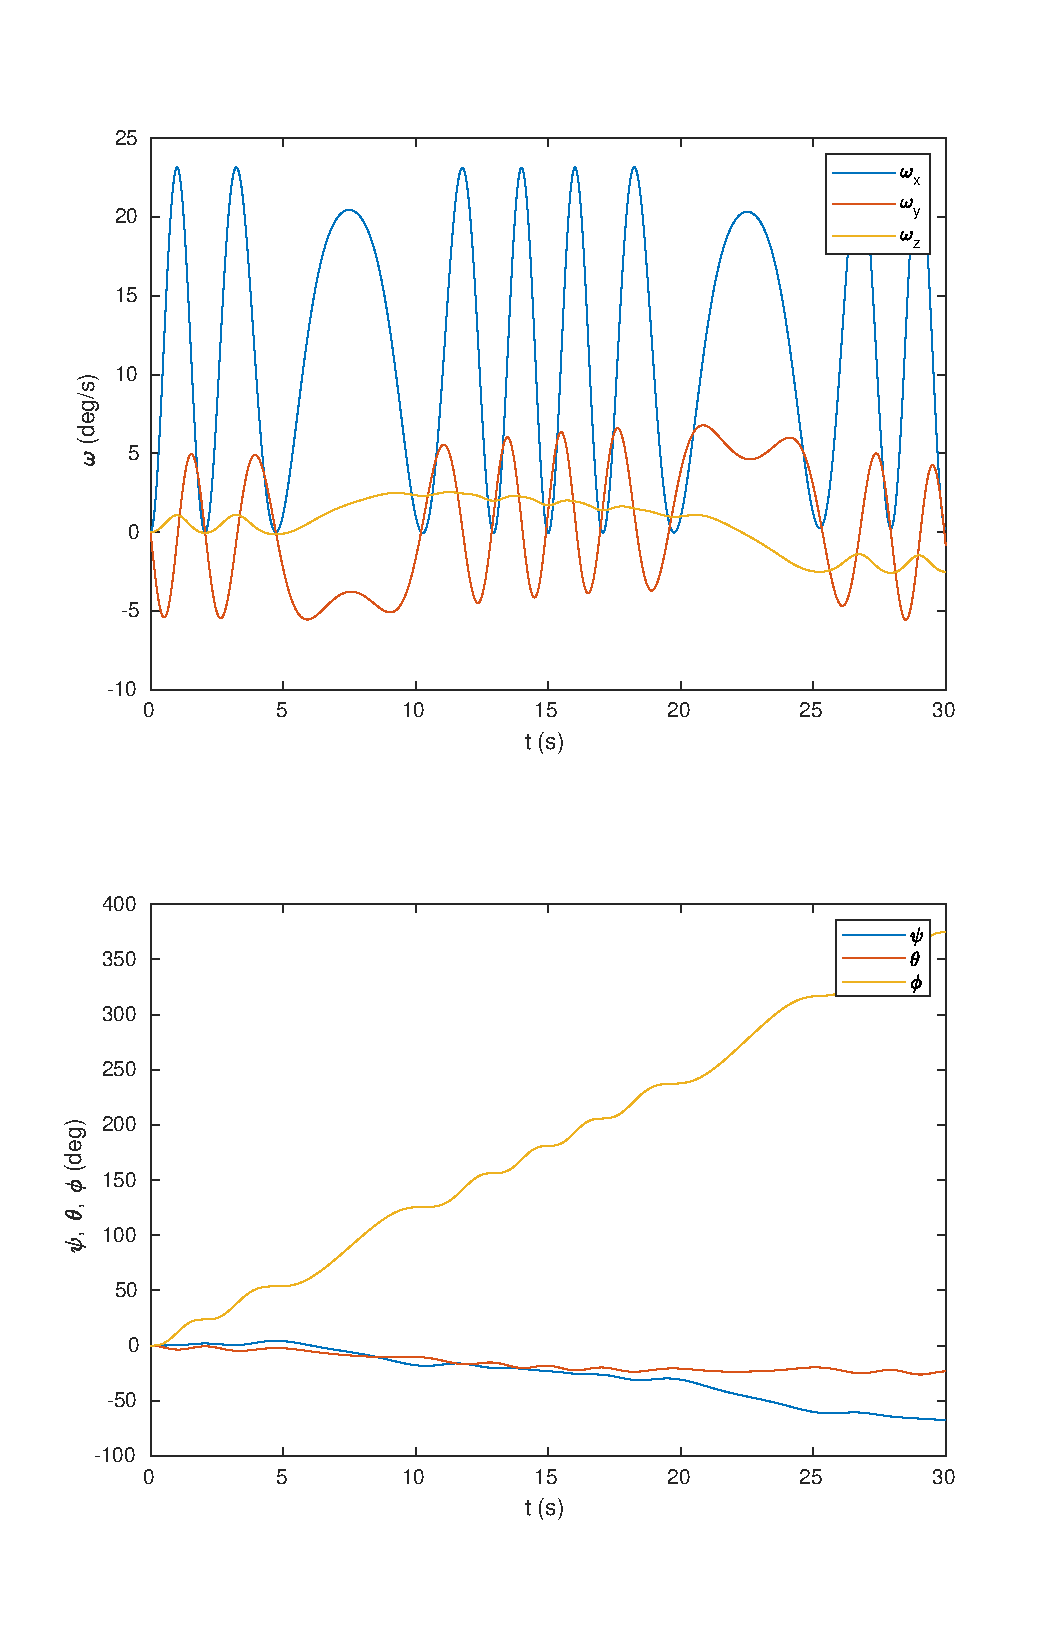
\includegraphics[scale=0.7]{task_e_b.eps}
    \end{center}
    \caption{Simulation of CSM attitude}
    \end{figure}
    Here is a table of maximum and minimum values
    \begin{table}[H]
      \centering
      \begin{tabular}{lcccccc}
        & $\omega_x$ & $\omega_y$ & $\omega_z$ & $\psi$ & $\theta$ & $\phi$ \\
        $\max$ &  0.4447 & 1.3419 & 0.0447 & 1.5270 & 0.0000 & 5.7141 \\
        $\min$ & -0.0034 & -1.3545 & 0 & -0.0259 & -12.9773 & 0.0000 \\
      \end{tabular}
      \caption{Table of max and min values shown in degrees and degrees per second}
    \end{table}
At first glance, these results look incorrect and nonsensical, however, they are correct due to the weirdness of 3D rotations. We note that
\[
  \left\{ \dot{\omega} \right\} = [I]^{-1} \left( \left\{ M \right\} - \left\{ \omega \right\} \times [I] \left\{ \omega \right\} \right)
\]
As expected at time zero, the quantities that immediately change are $\omega_y$ and $\theta$, since $\dot{H}_y \approx M_y \approx -I_R\Omega \dot{\theta_1}$. However as $\theta_1$ moves away from 0, we begin to get a positive $M_x$, due to the $s_{\theta_1}$ term. This induces a positive $\omega_x$. Now with rotation about two axes, the cross product $-\left\{\omega\right\} \times [I] \left\{ \omega \right\}$, has entries in the $z$ component, inducing a nonzero $\dot{\omega}_z$.
  \item With more complex inputs, we get the following motion
    \begin{figure}[H]
    \begin{center}
      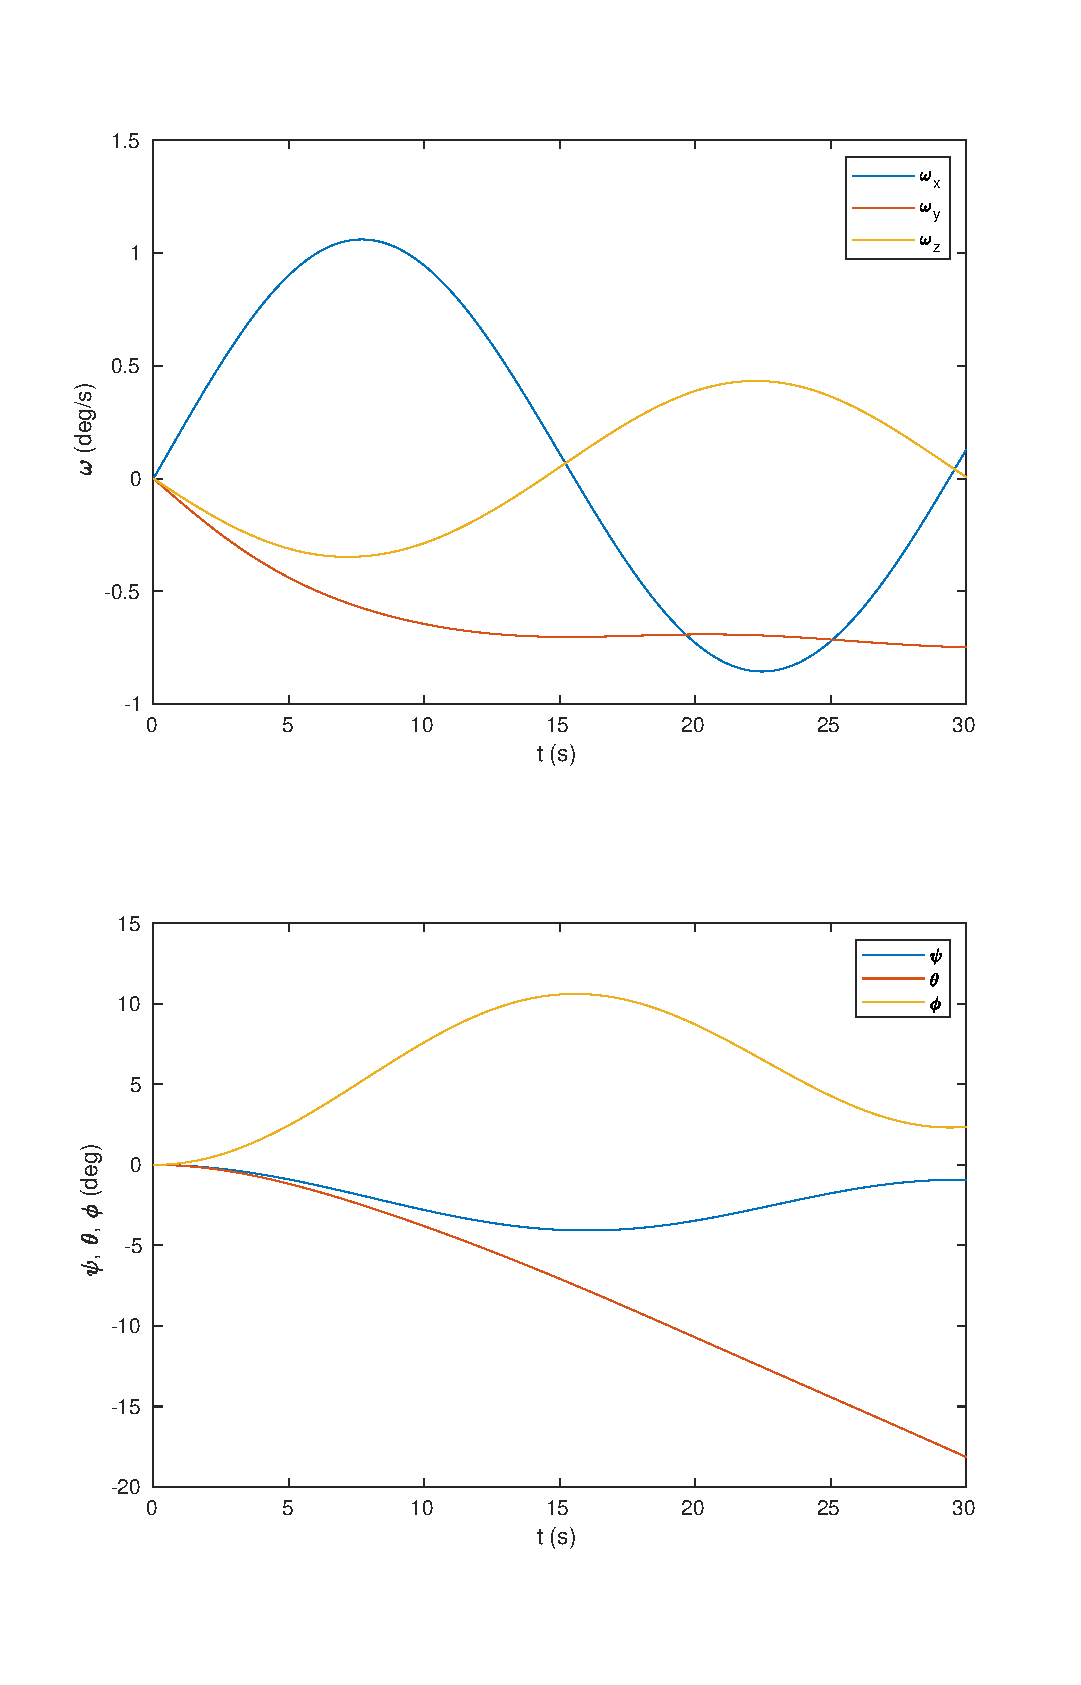
\includegraphics[scale=0.7]{task_e_c.eps}
    \end{center}
    \caption{Simulation of CSM attitude}
    \end{figure}
    Here is a table of maximum and minimum values
    \begin{table}[H]
      \centering
      \begin{tabular}{lcccccc}
        & $\omega_x$ & $\omega_y$ & $\omega_z$ & $\psi$ & $\theta$ & $\phi$ \\
        $\max$ &  1.0603 & 0 & 0.4329 & 0.0000 & 0.0000 & 10.6138 \\
        $\min$ & -0.8556 & -0.7485 & -0.3473 & -4.0726& -18.1336 & 0.0000 \\
      \end{tabular}
      \caption{Table of max and min values shown in degrees and degrees per second}
    \end{table}
\end{enumerate}

\section*{Task F:}%
It is well known that attitude evolves on the manifold $SO(3)$ and that all euler-angle combinations have singularities associated with certain attitudes. In such cases, it is more computationally efficient and safer to parameterize the attitude as a unit quaternion. It is well known that quaternions exhibit the following dynamics
\[
  \begin{aligned}
    \dot{q}_B^I &= \frac{1}{2} q_B^I \otimes  
  \begin{bmatrix}
    0 \\
    \omega
  \end{bmatrix} \\
    \dot{\omega} &= I^{-1} \left(M  - \omega \times I \omega\right)
  \end{aligned}
\]
Where $\otimes$ is the Hamilton quaternion product. Great care must be taken when integrating these equations, since we want the quaternion to stay on the manifold $SO(3)$. To do this, we can use the quaternion exponential
\[
  q^+ = q \otimes \exp \left( \begin{bmatrix}
    0 \\
    \omega \Delta t
  \end{bmatrix} \right)
\]
Where I have dropped the frames for brevity. Now we will design a PID-like controller with this new structure. Given a reference attitude quaternion $q_c$, we can define error in the following way
\[
  \delta q = \log \left( q_r \otimes q^* \right)
\]
where $*$ denotes the quaternion conjugate (inverse quaternion), and $\log$ is the inverse of the quaternion exponential. Now we can use successive loop closure ideas and say that the reference angular velocity is
\[
  \omega_r = K_{pq} \delta q + K_{dq} \dot{\delta q} + K_{iq} \int \delta q dt
\]
Now we need to design a control law based on $\theta_1, \theta_2, \theta_3$ and their derivatives to drive $\omega$ toward this reference. $M$ can be rewritten as  
\[
  M = -I_R \Omega 
  \begin{bmatrix}
    -s_{\theta_1} & 0 & c_{\theta_3} \\
    c_{\theta_1} & -s_{\theta_2} & 0\\
    0 & c_{\theta_2} & -s_{\theta_3}
  \end{bmatrix}
  \begin{bmatrix}
    \dot{\theta}_1 \\
    \dot{\theta}_2 \\
    \dot{\theta}_3
  \end{bmatrix}
\]
which is an invertible relationship whenever any two CMGs aren't aligned. In this way we have that
\[
  \begin{bmatrix}
    \dot{\theta}_1 \\
    \dot{\theta}_2 \\
    \dot{\theta}_3
  \end{bmatrix} =
  -\frac{1}{I_R \Omega} 
  \begin{bmatrix}
    -s_{\theta_1} & 0 & c_{\theta_3} \\
    c_{\theta_1} & -s_{\theta_2} & 0\\
    0 & c_{\theta_2} & -s_{\theta_3}
  \end{bmatrix}^{-1} M
\]

So given any $M$, we can choose CMG rates to command that $M$. Now we must decide how to choose $M$. Ideally we want something along the lines of
\[
  \dot{\omega} = K_{p\omega} \delta \omega + K_{d\omega} \dot{\delta \omega} + K_{i\omega} \int \delta \omega dt
\]
where $\delta \omega = \omega_r - \omega$, working from this base, we see that
\[
  M = \omega \times I \omega + I \left( K_p \delta \omega + K_d \dot{\delta \omega} + K_I \int \delta \omega dt \right)
\]
we note that the feedforward term $\omega \times I \omega$ is necessary in order to compensate for the change of momentum due to the rotation of the body frame.

This controller is implemented in \texttt{morris\_quat\_control.m} and the driver is given in \texttt{test\_driver\_quat\_control.m}. To avoid having to write my own quaternion library, I am using Peter Corke's robotics toolbox, so if you want to run my code, his toolbox will first need to be installed. Since quaternions are hard to visualize, I converted my plots back into euler angles. The test driver picks a random initial quaternion and a random commanded quaternion. It then calculates the control needed to move between those attitudes and performs the simulation. Some plots are shown below

\begin{figure}[H]
\begin{center}
  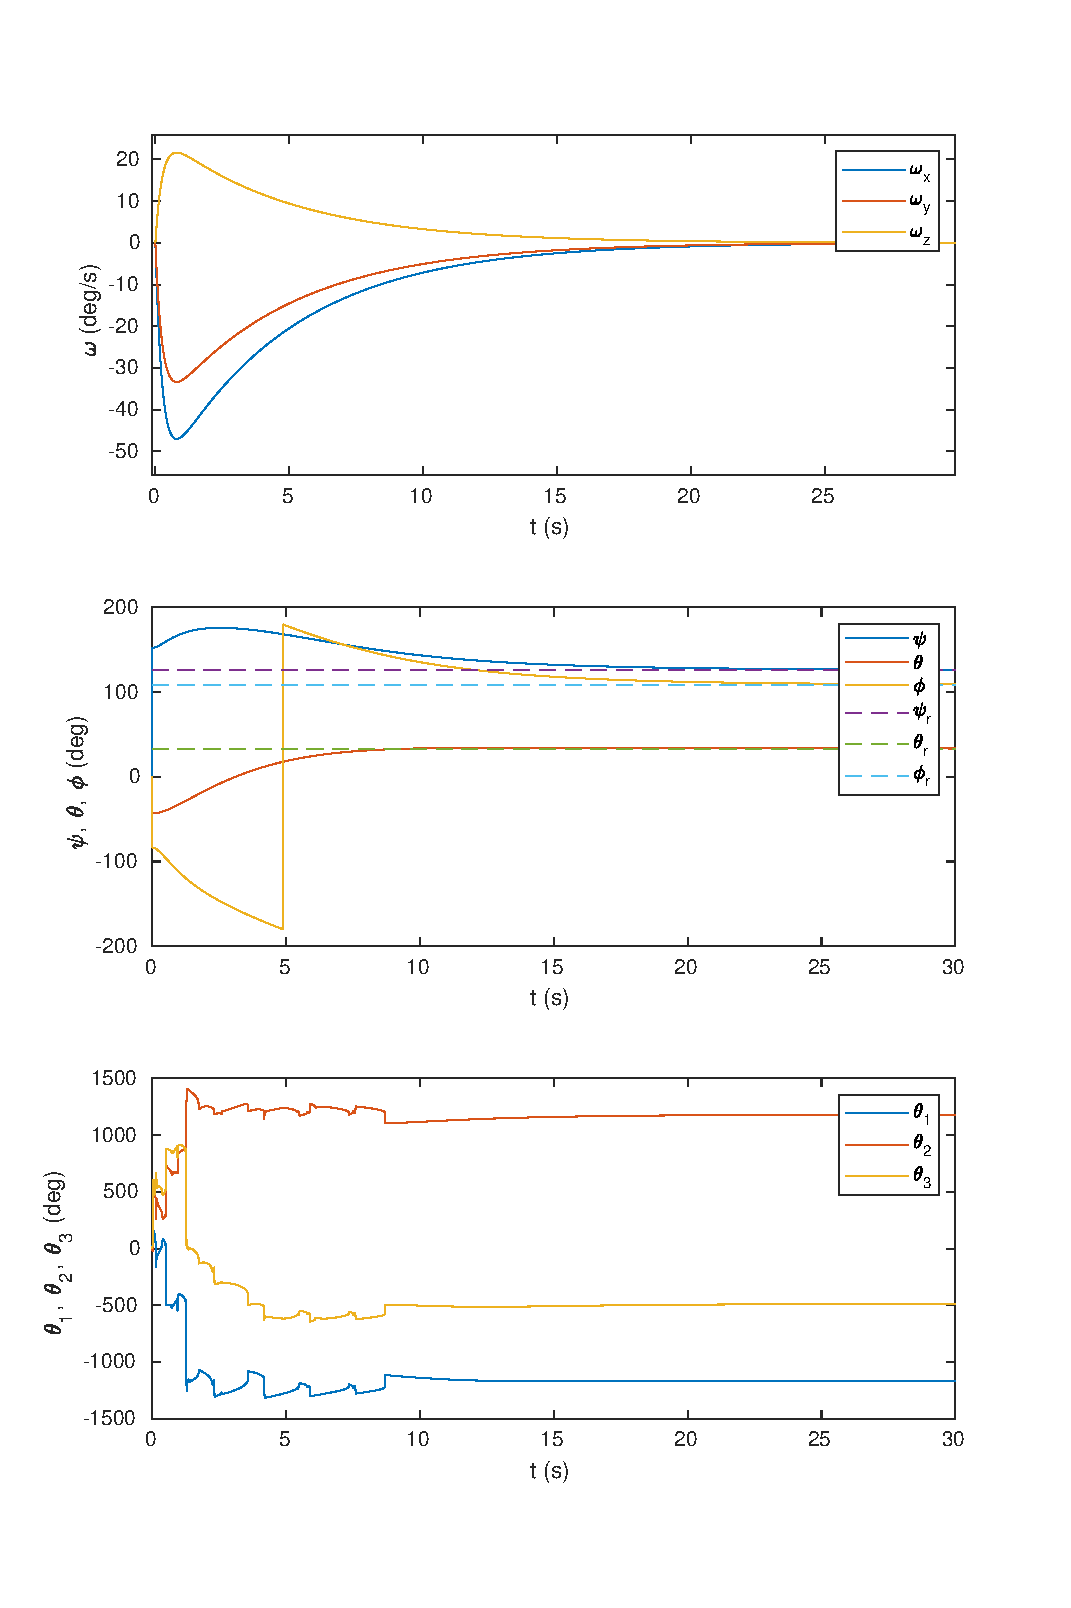
\includegraphics[scale=0.7]{task_f.eps}
\end{center}
\caption{Attitude Control of CSM (General)}
\label{fig:task_f}
\end{figure}

Some limitations of this simulation are that I did not model velocity constraints, joint contraints, or torque saturation limits on the CMGs. Looking at the $\theta$ plots, it's obvious that this is not a realistic scenario. Furthermore, there are moments when $\theta$ jumps. This is due to two CMGs being almost aligned and the matrix becomes almost singular. I did not explore strategies to prevent the CMGs from aligning their axes of rotation.

\end{document}
